\documentclass[12pt, oneside]{article}

\usepackage[letterpaper, scale=0.89, centering]{geometry}
\usepackage{fancyhdr}
\setlength{\parindent}{0em}
\setlength{\parskip}{1em}

\usepackage{tikz}
\usetikzlibrary{automata,positioning,arrows}

\pagestyle{fancy}
\fancyhf{}
\renewcommand{\headrulewidth}{0pt}
\rfoot{\href{https://creativecommons.org/licenses/by-nc-sa/2.0/}{CC BY-NC-SA 2.0} Version \today~(\thepage)}

\usepackage{amssymb,amsmath,pifont,amsfonts,comment,enumerate,enumitem}
\usepackage{currfile,xstring,hyperref,tabularx,graphicx,wasysym}
\usepackage[labelformat=empty]{caption}
\usepackage{xcolor}
\usepackage{multicol,multirow,array,listings,tabularx,lastpage,textcomp,booktabs}

% NOTE(joe): This environment is credit @pnpo (https://tex.stackexchange.com/a/218450)
\lstnewenvironment{algorithm}[1][] %defines the algorithm listing environment
{   
    \lstset{ %this is the stype
        mathescape=true,
        frame=tB,
        numbers=left, 
        numberstyle=\tiny,
        basicstyle=\rmfamily\scriptsize, 
        keywordstyle=\color{black}\bfseries,
        keywords={,procedure, div, for, to, input, output, return, datatype, function, in, if, else, foreach, while, begin, end, }
        numbers=left,
        xleftmargin=.04\textwidth,
        #1
    }
}
{}

\newcommand\abs[1]{\lvert~#1~\rvert}
\newcommand{\st}{\mid}

\newcommand{\cmark}{\ding{51}}
\newcommand{\xmark}{\ding{55}}


\begin{document}
\begin{flushright}
    \StrBefore{\currfilename}{.}
\end{flushright}

{\it Textbook references: Within a chapter, each item is numbered consecutively. Figure 1.22
is the twenty-second numbered item in chapter one; it comes right after Example 1.21 and right before Definition 1.23.}

In Computer Science, we operationalize ``hardest'' as ``requires most resources'', where
resources might be memory, time, parallelism, randomness, power, etc.
To be able to compare ``hardness'' of problems, we use a consistent description of problems

{\bf Input}: String

{\bf Output}: Yes/ No, where Yes means that the input string matches the pattern or property described by the problem.

So far: we saw that regular expressions are convenient ways of describring patterns in strings.
DFA give a model of computation for processing strings and and classifying them into Yes (accepted)
or No (rejected). We will see that each set of strings is described by a regular expression if and only 
if there is a DFA that recognizes it.  Another way of thinking about it: properties described by regular
expressions require exactly the computational power of DFAs.


\section*{Monday April 4}

%! app: regular-languages
%! outcome: Regular expressions, Formal definition of automata, Informal definition of automata


{\bf Review}: Formal definition of DFA: $M = (Q, \Sigma, \delta, q_0, F)$ 

\begin{center}
\begin{multicols}{2}
\begin{itemize}
\setlength{\itemsep}{2pt}
\item Finite set of states $Q$
\item Alphabet $\Sigma$
\item Transition function $\delta$
\item Start state $q_0$
\item Accept (final) states $F$
\end{itemize}
\end{multicols}
\end{center}
In the state diagram of $M$, how many outgoing arrows are there from each state?

$M = ( \{ q, r, s\}, \{a,b\}, \delta, q, \{s\} )$ 
where $\delta$ is  (rows labelled by states
and columns labelled by symbols):
\begin{center}
\begin{tabular}{c|cc}
$\delta$ & $a$ & $b$ \\
\hline
$q$ & $r$ & $q$ \\
$r$ & $r$ & $s$ \\
$s$ & $s$ & $s$ \\
\end{tabular}
\end{center}

The state diagram for $M$ is 

\vfill



Give two examples of strings that are accepted by $M$ and two examples of strings that are rejected by $M$:

\vfill

Add ``labels" for states in the state diagram, e.g. ``have not seen any of desired pattern yet'' or
``sink state''.
\newpage

We can use the analysis of the roles of the states in the state diagram to describe the language
recognized by the DFA. 


$L(M) = $

A regular expression describing $L(M)$ is




\vspace{300pt}

Let the alphabet be $\Sigma_1 = \{0,1\}$.

A state diagram for a DFA that recognizes $\{w \mid w~\text{contains at most two $1$'s} \}$ is

\vspace{70pt}

A state diagram for a DFA that recognizes $\{w \mid w~\text{contains more than two $1$'s} \}$ is

\vspace{70pt}


\newpage
{\it Extra example:} A state diagram for DFA recognizing
$$\{w \mid w~\text{is a string over $\{0,1\}$ whose length is not a multiple of $3$} \}$$

\vspace{70pt}


Let $n$ be an arbitrary positive integer. What is a formal definition for a DFA recognizing
\[
\{w \mid w~\text{is a string over $\{0,1\}$ whose length is not a multiple of $n$} \}?
\]

\vspace{70pt}
    
\newpage
\subsection*{Review: Week 2 Monday}

Please complete the review quiz questions on \href{http://gradescope.com}{Gradescope} about 
the languages recognized by DFAs.


Recall: Review quizzes based on class material are assigned each day. 
These quizzes will help you track and confirm your understanding of the concepts and examples 
we work in class. Quizzes can be submitted on Gradescope as many times (with no penalty) as 
you like until the quiz deadline: the three quizzes each week are all due on Friday (with no penalty 
late submission open until Sunday).

{\bf Pre class reading for next time}: Pages 45-47.


\newpage
\subsection*{Wednesday April 6}

%! app: Regular Languages
%! outcome: Regular expressions, Formal definition of automata, Informal definition of automata

Suppose A is a language over an alphabet $\Sigma$. By definition, this means A is a subset of $\Sigma^*$.
{\bf Claim:} if there is a DFA $M$ such that $L(M) = A$ then there is another DFA, let's call it $M'$, such that 
$L(M') = \overline{A}$, the complement of $A$, defined as $\{ w \in \Sigma^* \mid w \notin A \}$.

{\bf Proof idea}:


{\bf Proof}: 




\vfill
A useful (optional) bit of terminology: the {\bf iterated transition function} of a DFA
$M = (Q, \Sigma, \delta, q_0, F)$ is defined recursively by
\[
\delta^* (~(q,w)~) 
=\begin{cases}
q  \qquad &\text{if $q \in Q, w = \varepsilon$} \\
\delta( ~(q,a)~) \qquad &\text{if $q \in Q$, $w = a \in \Sigma$ } \\
\delta(~(\delta^*(q,u), a) ~) \qquad &\text{if $q \in Q$, $w = ua$ where $u \in  \Sigma^*$ and $a \in \Sigma$}
\end{cases}
\]

Using  this terminology, $M$ accepts a string $w$ over $\Sigma$ if and only if $\delta^*( ~(q_0,w)~) \in F$.

\newpage

Fix  $\Sigma = \{a,b\}$. A state diagram for a DFA that recognizes 
$\{w \mid w~\text{has $ab$ as a substring and is of even length} \}$:


\vspace{120pt}


Suppose $A_1, A_2$ are languages over an alphabet $\Sigma$.
{\bf Claim:} if there is a DFA $M_1$ such that $L(M_1) = A_1$ and 
DFA $M_2$ such that $L(M_2) = A_2$, then there is another DFA, let's call it $M$, such that 
$L(M) = A_1 \cap A_2$.

{\bf Proof idea}:


{\bf Formal construction}: 


\vspace{70pt}

{\bf Application}:  When $A_1 = \{w \mid w~\text{has $ab$ as a substring} \}$ and 
$A_2 = \{ w \mid w~\text{is of even length} \}$.


\newpage

Suppose $A_1, A_2$ are languages over an alphabet $\Sigma$.
{\bf Claim:} if there is a DFA $M_1$ such that $L(M_1) = A_1$ and 
DFA $M_2$ such that $L(M_2) = A_2$, then there is another DFA, let's call it $M$, such that 
$L(M) = A_1 \cup A_2$.  {\it Sipser Theorem 1.25, page 45}

{\bf Proof idea}:


{\bf Formal construction}: 

\vspace{70pt}

{\bf Application}: A state diagram for a DFA that recognizes $\{w \mid w~\text{has $ab$ as a substring or is of even length} \}$:

\vspace{100pt}


\newpage
\subsection*{Review: Week 2 Wednesday}

Please complete the review quiz questions on \href{http://gradescope.com}{Gradescope} about 
the languages recognized by DFAs.


Recall: Review quizzes based on class material are assigned each day. 
These quizzes will help you track and confirm your understanding of the concepts and examples 
we work in class. Quizzes can be submitted on Gradescope as many times (with no penalty) as 
you like until the quiz deadline: the three quizzes each week are all due on Friday (with no penalty 
late submission open until Sunday).


{\bf Pre class reading for next time}: Introduction to Section 1.2

\newpage
\subsection*{Friday April 8}

%! app: regular-languages
%! outcome: Formal definition of automata, Informal definition of automata, Nondeterminism


\begin{center}
\begin{tabular}{|ll|}
\hline
\multicolumn{2}{|l|}{{\bf Nondeterministic finite automaton} $M = (Q, \Sigma, \delta, q_0, F)$} \\
Finite set of states $Q$  & Can  be labelled by any collection  of distinct names. Default: $q0, q1, \ldots$  \\
Alphabet $\Sigma$ &  Each input to the automaton is a string over  $\Sigma$. \\
Arrow labels $\Sigma_\varepsilon$ &  $\Sigma_\varepsilon = \Sigma \cup \{ \varepsilon\}$. \\
&  Arrows 
in the state diagram are labelled either by symbols from $\Sigma$ or by $\varepsilon$ \\
Transition function $\delta$  & $\delta: Q \times \Sigma_{\varepsilon} \to \mathcal{P}(Q)$
gives the {\bf set of possible next states} for a transition \\
&  from the current state upon reading a symbol or spontaneously moving.\\
Start state $q_0$ & Element of $Q$.  Each computation of the machine starts at the  start  state.\\
Accept (final) states $F$ & $F \subseteq  Q$.\\
$M$ accepts the input string & if and only if {\bf there is} a computation of $M$ on the input string\\
&  that 
processes the whole string and ends in an
accept state.\\
\hline
{\it Page 53}& \\
\hline
\end{tabular}
\end{center}

The formal definition of the NFA over $\{0,1\}$ given by this state diagram is: 

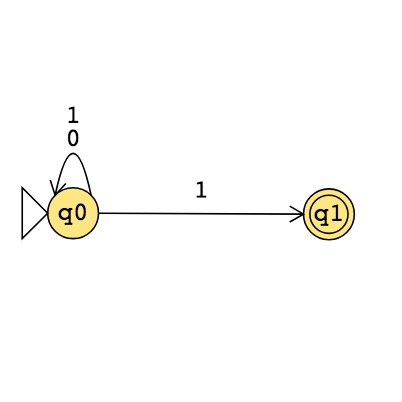
\includegraphics[width=2in]{../../resources/machines/Lect4NFA1.png}

The language over $\{0,1\}$ recognized by this NFA is:

\vspace{70pt}

Change the transition function to get a different NFA which accepts
the empty string.


\newpage

The state diagram of an NFA over $\{a,b\}$ is below.  The formal definition of this NFA is:

\vspace{-30pt}

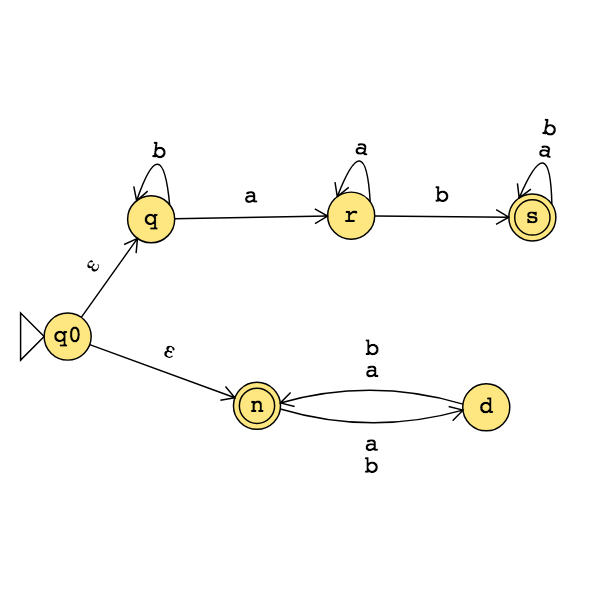
\includegraphics[width=2.5in]{../../resources/machines/Lect5NFA1.png}


\vspace{-10pt}

The language recognized by this NFA is: 


\newpage

\subsection*{Review: Week 2 Friday}


Please complete the review quiz questions on \href{http://gradescope.com}{Gradescope} about 
NFA.

{\bf Pre class reading for next time}: Theorem 1.47, Theorem 1.49

\end{document}